\chapter{Intro to Vectors and Matrices}

Given $\vec{a} = \begin{bmatrix} -2 \\ 1 \end{bmatrix}$ and $\vec{b} = \begin{bmatrix} 3 \\ 0 \end{bmatrix}$, find and sketch the result of each.

\begin{multicols}{5}
\begin{enumerate}
	\item $\vec{a} + \vec{b}$
	\item $\vec{a} - \vec{b}$
	\item $2\vec{a}$
	\item $3\vec{b} $
	\item $2\vec{a} + 3\vec{b}$
\end{enumerate}	\setcounter{Review}{\value{enumi}}
\end{multicols}

\newpage

\section{Answer Key}

\begin{enumerate}
	\item $\begin{bmatrix} 1 \\ 1 \end{bmatrix}$ \newline\\
    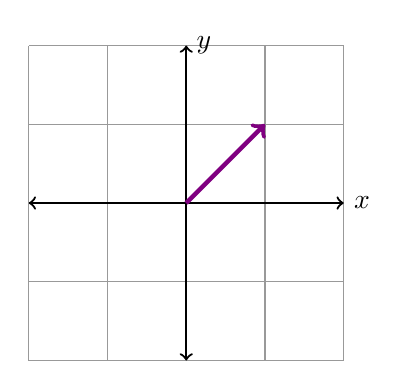
\begin{tikzpicture}
    \draw [gray!80] (-2,-2) grid (2,2);
    \draw[<->, thick] (-2,0) -- (2,0) node [right] {$x$};
    \draw[<->, thick] (0,-2) -- (0,2) node [right] {$y$};
    \draw[ultra thick, violet, ->] (0,0) -- (1,1);
    \end{tikzpicture}
    
    \item $\begin{bmatrix} -5 \\ 1 \end{bmatrix}$ \newline\\
    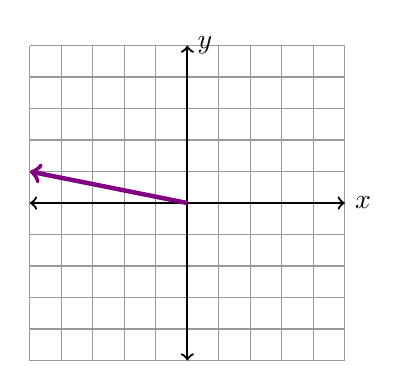
\begin{tikzpicture}[scale=0.4]
    \draw [gray!80] (-5,-5) grid (5,5);
    \draw[<->, thick] (-5,0) -- (5,0) node [right] {$x$};
    \draw[<->, thick] (0,-5) -- (0,5) node [right] {$y$};
    \draw[ultra thick, violet, ->] (0,0) -- (-5,1);
    \end{tikzpicture}
    
    \item $\begin{bmatrix} -4 \\ 2 \end{bmatrix}$ \newline\\
    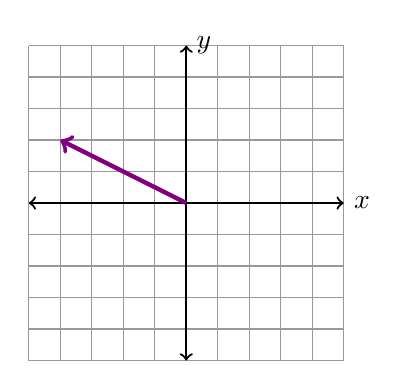
\begin{tikzpicture}[scale=0.4]
    \draw [gray!80] (-5,-5) grid (5,5);
    \draw[<->, thick] (-5,0) -- (5,0) node [right] {$x$};
    \draw[<->, thick] (0,-5) -- (0,5) node [right] {$y$};
    \draw[ultra thick, violet, ->] (0,0) -- (-4,2);
    \end{tikzpicture}
    
    \item $\begin{bmatrix} 9 \\ 0 \end{bmatrix}$ \newline\\
    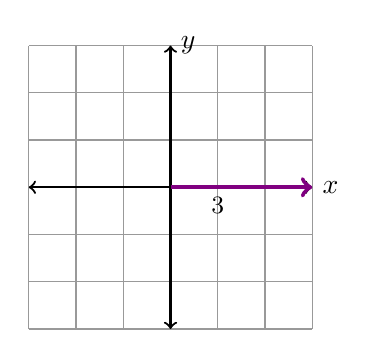
\begin{tikzpicture}[scale=0.6]
    \draw [gray!80] (-3,-3) grid (3,3);
    \draw[<->, thick] (-3,0) -- (3,0) node [right] {$x$};
    \draw[<->, thick] (0,-3) -- (0,3) node [right] {$y$};
    \node at (1,0) [below] {\small 3};
    \draw[ultra thick, violet, ->] (0,0) -- (3,0);
    \end{tikzpicture}
    
    \item $\begin{bmatrix} 5 \\ 2 \end{bmatrix}$ \newline\\
    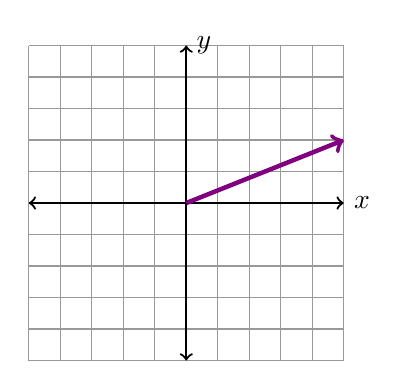
\begin{tikzpicture}[scale=0.4]
    \draw [gray!80] (-5,-5) grid (5,5);
    \draw[<->, thick] (-5,0) -- (5,0) node [right] {$x$};
    \draw[<->, thick] (0,-5) -- (0,5) node [right] {$y$};
    \draw[ultra thick, violet, ->] (0,0) -- (5,2);
    \end{tikzpicture}
\end{enumerate}